\subsection{SLAM Testing}
\label{subsec:slamtesting}

\begin{figure} [ht]
  \centering
  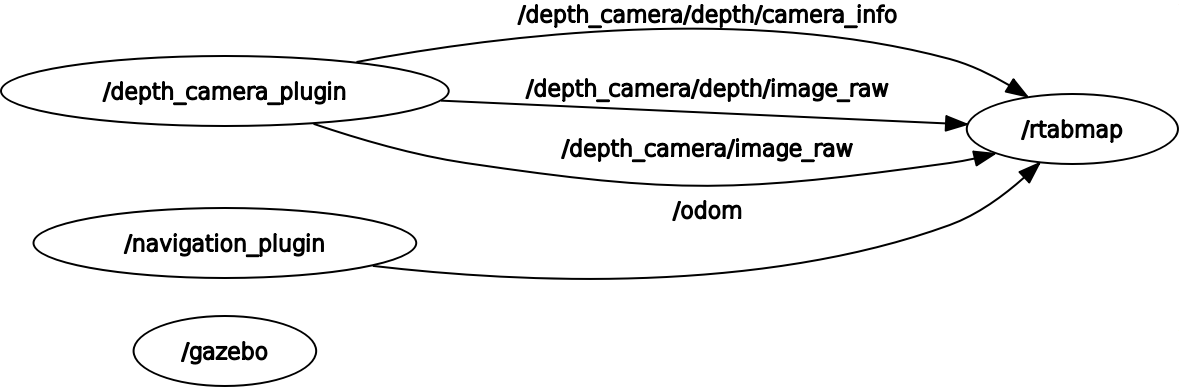
\includegraphics[width=0.45\textwidth]{figures/rosgraph/slam.png}
  \IfLanguageName{english}{
    \caption{Node scheme of the SLAM testing.}
  }{
    \caption{Skema \emph{node} dari pengujian SLAM.}
  }
  \label{fig:rosgraphslam}
\end{figure}


SLAM (simultaneous localization and mapping) Testing is done in the simulation with purpose to test the virtual room ability in simulating the real room.
In this test,
  the robot model will move around the room while doing the mapping using the SLAM method.
As shown in the figure \ref{fig:rosgraphslam},
  \lstinline{rtabmap} node will be connected to the \lstinline{depth_camera_plugin} node and the \lstinline{navigation_plugin} node that will send color image, depth image, and odometry data which will be used in the room mapping process.

\begin{figure} [ht]
  \centering
  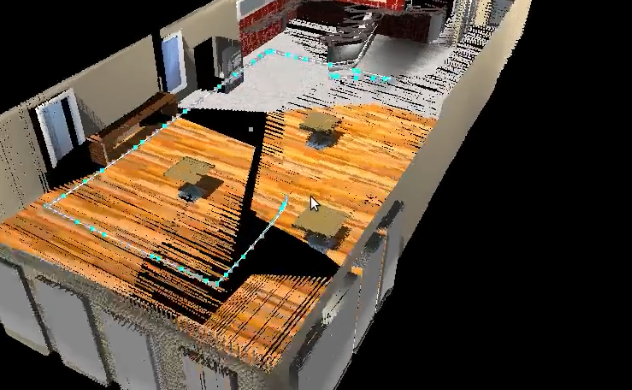
\includegraphics[width=0.4\textwidth]{figures/slam.png}
  \IfLanguageName{english}{
    \caption{Room mapping results.}
  }{
    \caption{Hasil pemetaan ruangan.}
  }
  \label{fig:slam}
\end{figure}


The result,
  as shown in the figure \ref{fig:slam},
  the room mapping process produce a three-dimensional map that composed of point clouds which shape the room that is tested in the simulation.
That map is displayed on the GUI that owned by the \lstinline{rtabmap} node.
Besides that,
  The map also shows a visualization of the path that the robot has traversed as a line with a blue dot.
